\documentclass[aspectratio=169]{beamer}
% \RequirePackage[T2A]{fontenc}

\usepackage{listings}
\usepackage{courier}
\usepackage{tikz}
\usepackage{tikz-qtree}
\usepackage{algorithmic}
\usepackage{algorithm}
\usepackage{float}
\usepackage{graphicx}
\usepackage{epstopdf}
\usepackage{longtable}

%\usepackage{algorithm2e}

\usetikzlibrary{shapes,arrows}

%\usetheme{CambridgeUS}%{Warsaw}
%\usetheme {Madrid}
%\useoutertheme {shadow}
%\usecolortheme{beaver}%{structure черный}%{seagull серый}%{lily желтый}%{beaver красный}
%\usefonttheme{structurebold}
%\setbeamerfont{framesubtitle}{size=\large}
%\useoutertheme{infolines}
%\useoutertheme{split}
%I DONT WANT TO SEE THOSE NAVIGATION SYMBOLS
%\setbeamertemplate{navigation symbols}{}

% \mode<presentation>
% {
%     \usefonttheme[onlymath]{serif}
% \usetheme {Madrid}
% %\useoutertheme {shadow}
% %\usecolortheme{volverine}%{structure черный}%{seagull серый}%{lily желтый}%{beaver красный}
% \usefonttheme{structurebold}
% \setbeamerfont{framesubtitle}{size=\large}
% \useoutertheme{infolines}
% %\useoutertheme{split}
% %I DONT WANT TO SEE THOSE NAVIGATION SYMBOLS
% \setbeamertemplate{navigation symbols}{}
% \setbeamertemplate{footline}
% }
\usetheme{Warsaw}
\usecolortheme{crane}
\beamertemplatenavigationsymbolsempty

\hypersetup{
    bookmarks=true,         % show bookmarks bar?
    unicode=true,           % non-Latin characters in Acrobat’s bookmarks
    pdftoolbar=false,        % show Acrobat’s toolbar?
    pdfmenubar=false,        % show Acrobat’s menu?
    pdffitwindow=false,     % window fit to page when opened
    pdfstartview={FitH},    % fits the width of the page to the window
    pdftitle={Компьютерная алгебра в задачах оптимизации},    % title
    pdfauthor={Evgeny Cherkashin, Seseg Badmatsyrenova},     % author
    pdfsubject={symbolic computations},   % subject of the document
    pdfnewwindow=true,      % links in new PDF window
    colorlinks=true,       % false: boxed links; true: colored links
    linkcolor=red,          % color of internal links (change box color with linkbordercolor)
    citecolor=green,        % color of links to bibliography
    filecolor=magenta,      % color of file links
    urlcolor=blue           % color of external links
}

\usepackage{iftex,ifxetex}
\ifPDFTeX
  \usepackage[utf8]{inputenc}
  %\usepackage[T1]{fontenc}
  %\usepackage[russian]{babel}
  \usepackage{lmodern}
  \usefonttheme{serif}
\else
  \ifluatex
    \usepackage{unicode-math}
    \defaultfontfeatures{Ligatures=TeX,Numbers=OldStyle}
    \setmathfont{Latin Modern Math}
    \setsansfont{Linux Biolinum O}
    \usefonttheme{professionalfonts}
    \setmathfont[
        Ligatures=TeX,
        Scale=MatchLowercase,
        math-style=upright,
        vargreek-shape=unicode
        ]{euler.otf}
  \fi
\fi


%\setbeamercolor{color1}{bg=red!40!green,fg=black}
%\setbeamercolor{uppercol}{fg=white,bg=brown}
%\setbeamertemplate{background canvas}[vertical shading][bottom=white!80!cyan!20,top=cyan!10]

\title{Positive Constructed Formulas Preprocessing\\ for Automatic Deduction}

\author[A.~Davydov]{\textbf{Artem~Davydov}, \textbf{Alexander~Larionov}, \underline{Evgeny~Cherkashin}, Savely~Arlyapov\\\texttt{\scriptsize{ethrik@gmail.com, bootfrost@zoho.com eugeneai@icc.ru}}}


\institute[ISDCT SB RAS, INRTU]
{Matrosov Institute for System Dynamics and Control Theory of Siberian Branch of Russian Academy of Sciences; \\[0.5em]
Irkutsk National Research Technical University,\\
Irkutsk, Russian Federation
}

\date{\scriptsize{
\\
    \vspace{0.3cm}}
ISDCT SB RAS, INRTU
\\
31 May 2016
\\
Opatija, Croatia
}
\begin{document}
\maketitle{}
\newpage
\begin{frame}

\frametitle{Introduction: Automated Theorem Proving}
\begin{block}{Automated theorem proving (ATP)}
ATP is a part of artificial intelligence; it is based on methods of mathematical logic and realized as computer programs called provers (or solvers, or systems of ATP).
\end{block}
\begin{block}{Theorem}
<<Theorem>> describes a domain and a problem to be solved on some logical language (predicate language, clause language etc.).
\end{block}
\begin{block}{Prover}
A prover finds out whether some formula is a theorem.
\end{block}
\end{frame}

\begin{frame}

\frametitle{Introduction: Application of provers}

\begin{enumerate}
\item Solving of mathematical problems. There are examples of solving some open mathematical problems\footnote{W.McCune. Solution of the Robbins problem;};
\item Software and hardware verification;
\item Program synthesis;
\item Expert systems;
\item Problem solving;
\item There are examples of the provers in areas of natural language processing, computer vision etc.
\end{enumerate}
\begin{block}{}
The most famous and efficient provers: Vampire, E, Prover9, Otter, SPASS, EQP, Isabelle, ACL2 etc.
\end{block}
\end{frame}

\begin{frame}
\frametitle{Features of PCF}
The PCF calculus is both \textbf{machine-oriented}, and \textbf{human-oriented}, naturally it was aimed at solving the problems of \textbf{control of dynamic systems}.

Features of PCFs follows:
\begin{enumerate}
\item unique inference rule and simple scheme of axioms;
\item modifyability
  of semantics (constructive, monotonic, temporal, etc.);
\item
  it is possible to construct intuitionistic inferences of some
  non-Horn formulas;
\item explicit usage of $\forall$-- and
  $\exists$--quantifiers;
\item scolemization procedure is not required.

\end{enumerate}
The calculi of PCFs preserve heuristic structure of the original PC\footnote{Predicate calculus.} presentation of the theorem to be proved.
\end{frame}

\begin{frame}

\frametitle{Positively Constructed Formulae: an example}

\begin{figure}
\includegraphics[width=0.8\linewidth]{pics/ex1}
\end{figure}

\end{frame}

%%----------example 2--------------
\begin{frame}
\frametitle{Positively Constructed Formulae: Semantics}
\begin{figure}
\includegraphics[width=0.8\linewidth]{pics/branching}
\end{figure}

\end{frame}


%%----METHODS--------
\begin{frame}

\frametitle{Research in the field}
The research deals with adopting various nowadays techniques such as:
\begin{itemize}
\item data structures for formulae representation;
\item sharing of data structures, garbage collection;
\item efficient structure manipulation;
\item term indexing (relations: inst/2, gen/2, unif/2, var/2);
\item inference search process control and guiding;
\item parallel implementations of the inference rule;
\item testing on TPTP library of first--order theorems.
\end{itemize}
Application areas are (a little progress):
\begin{itemize}
\item Logical driven imitation modeling;
\item Control synthesis;
\item PCFs based programming language.
\end{itemize}
\end{frame}

%%----------Methods----------
\begin{frame}

\frametitle{Formal part: PC to PCF conversion}
\begin{block}{source predicate calculus formula}
$$F = \forall x\forall y(S(x,y)\leftrightarrow\forall z(I(z,x)\rightarrow I(z,y))).$$
\end{block}
The transformations should preserve a heuristic structure of the original formula.
\begin{block}{Connection $\leftrightarrow$ and $\to$ elimination}
$$\begin{array}{l}
F = \forall x\forall y( F_1 \& F_2 );\\
\quad F_1 = \neg S(x,y)\vee\forall z(\neg I(z,x)\vee I(z,y));\\
    \quad F_2 = \neg\forall z(\neg I(z,x)\vee I(z,y)) \vee S(x,y) =\\
    \quad F_2^\prime = \exists z( I(z,x)\&\neg I(z,y) ) \vee S(x,y).
\end{array}
$$
\end{block}
\end{frame}

\begin{frame}

\frametitle{PC to PCF conversion}
\begin{block}{Translated formula}
\begin{center}
\Tree[. $\forall x$ [. $\forall y$ [. $\&$ $F_1$ $F_2$ ] ] ]
\Tree[. \hspace{5mm} ]
\Tree[. $F_1$ [. $\vee$ $\neg S(x,y)$ [. $\forall z$ [. $\vee$ $\neg I(z,x)$ $I(x,y)$ ] ] ] ]
\Tree[. $F_2$ [. $\vee$ [. $\exists z$ [. $\&$ $I(z,x)$ $\neg I(z,y)$ ] ] $S(x,y)$ ] ]
\end{center}
\end{block}
\end{frame}

\begin{frame}
\frametitle{Conversion algorithm (FOL $\to$ PCF) $F^\pi(N)^P$}
%\begin{block}{}
\renewcommand{\algorithmicrequire}{\textbf{Input:}}
\renewcommand{\algorithmicensure}{\textbf{Output:}}
\begin{figure}[H]
  \footnotesize\centering
%\begin{algorithm}
% %\caption{FOF to PCF conversion algoritm}\label{alg:conv}
\begin{algorithmic}
  \REQUIRE Node $N$ is the root of a tree $T$ for $F$; \\
  $P \in \{\forall,\exists\}$, $P=\forall$ by default.
\ENSURE $F^{\pi}$ is a PCF image of FOL $F$.
\IF [Node $N$ has children.] {$N = Qx \& P\neq Q$}
\RETURN  $F^{\pi} = Qx\colon\varnothing ( (G_{N'}^{\pi})^{P} )$
\ENDIF
\IF [Node $N$ has children.] {$N=\vee$}
  \RETURN  $F^{\pi} = \forall\varnothing \bigl( (G_{N'_1}^{\pi})^{\exists},\ldots,(G_{N'_k}^{\pi})^{\exists}\bigr)$
\ENDIF
\IF [Node $N$ has children.] {$N=\&$}
  \RETURN  $F^{\pi} = \exists\varnothing \bigl( (G_{N'_1}^{\pi})^{\forall},\ldots,(G_{N'_k}^{\pi})^{\forall}\bigr)$
\ENDIF
\IF[$R$ is an atom] {$N=R$}
  \RETURN  $F^{\pi} = \exists\varnothing\colon R$
\ENDIF
\IF[$R$ is an atom] {$N=\neg R$}
  \RETURN  $F^{\pi} = \forall\varnothing\colon R$
\ENDIF
\end{algorithmic}
%\end{algorithm}
\end{figure}
%\end{block}
%\begin{figure}
%\includegraphics[scale=0.45]{pics/pic3}
%\caption{path indexing}
\end{frame}

\begin{frame}
\frametitle{Result of conversion for our example}
%\begin{figure}
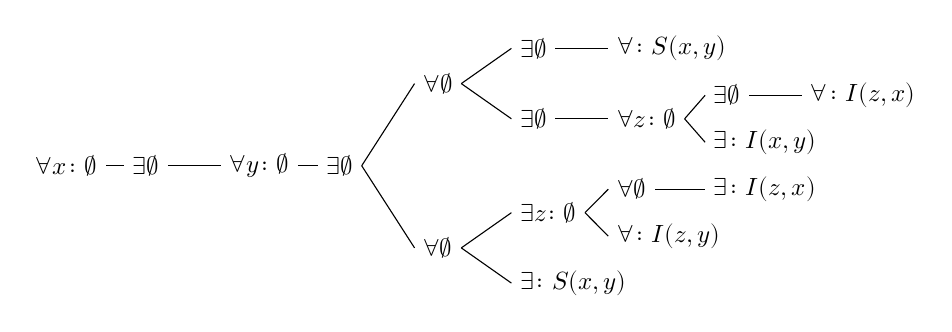
\begin{tikzpicture} \small
\tikzset{grow'=right}
%\tikzset{execute at begin node=\strut}
\tikzset{level distance=35pt}
\tikzset{every tree node/.style={align=left,anchor=west}}
\Tree [. $\forall x\colon\varnothing$ [. $\exists\varnothing$ [. $\forall y\colon\varnothing$ [. $\exists\varnothing$
[. $\forall\varnothing$ [. $\exists\varnothing$ $\forall\colon S(x,y)$ ]
			[. $\exists\varnothing$ [. $\forall z\colon\varnothing$ [. $\exists\varnothing$  $\forall\colon I(z,x)$ ] $\exists\colon I(x,y)$  ] ] ]
[. $\forall\varnothing$ [. $\exists z\colon\varnothing$ [. $\forall\varnothing$ $\exists\colon I(z,x)$ ] $\forall\colon I(z,y)$ ] $\exists\colon S(x,y)$ ] ] ] ] ]
\end{tikzpicture}
% \end{figure}

Now, the formula is to be reduced.
\end{frame}

%%----------Methods----------
\begin{frame}

\frametitle{Theorem: Reduction rule}
\begin{block}{Input}
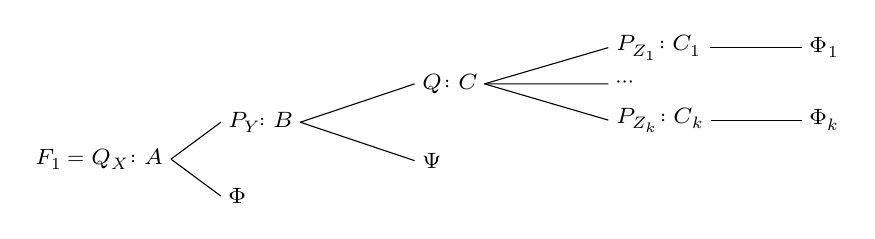
\begin{tikzpicture}\footnotesize\centering
\tikzset{grow'=right}
%\tikzset{execute at begin node=\strut}
\tikzset{level distance=70pt}
\tikzset{every tree node/.style={align=left,anchor=west}}
\Tree [. $F_1=Q_X\colon A$ [. $P_Y\colon B$ [. $Q\colon C$ [. $P_{Z_1}\colon C_1$ $\Phi_1$ ] $\cdots$ [. $P_{Z_k}\colon C_k$ $\Phi_k$ ] ] $\Psi$ ] $\Phi$ ]
\end{tikzpicture}
\end{block}

Quantifiers $P,Q\in\{\forall,\exists\}, P\neq Q$, $A,C,B$ are conjunctions, $C\subseteq B$, $\Phi,\Psi,\Phi_i$ are sets of formulae. After conversion $F_2\leftrightarrow F_1$.

\begin{block}{Result}\footnotesize
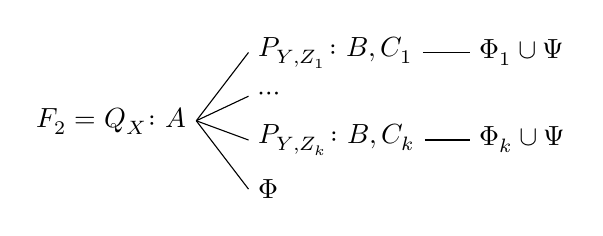
\begin{tikzpicture}
\tikzset{grow'=right}
%\tikzset{execute at begin node=\strut}
\tikzset{level distance=80pt}
\tikzset{every tree node/.style={align=left,anchor=west}}
\Tree [. $F_2=Q_X\colon A$ [. $P_{Y,Z_1}\colon B,C_1$ $\Phi_1\cup\Psi$ ] $\cdots$ [. $P_{Y,Z_k}\colon B,C_k$ $\Phi_k\cup\Psi$ ] $\Phi$ ]
\end{tikzpicture}
\end{block}
\end{frame}

%%----------Methods----------
\begin{frame}

\frametitle{Reduction rule applied to the example}
\begin{block}{Reduced PCF}
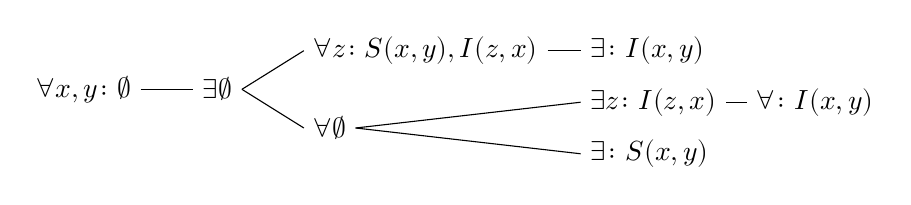
\begin{tikzpicture}
\tikzset{grow'=right}
%\tikzset{execute at begin node=\strut}
%\tikzset{level distance=70pt}
\tikzset{level 1/.style={level distance=60pt}}
\tikzset{level 2/.style={level distance=40pt}}
\tikzset{level 3/.style={level distance=100pt}}
\tikzset{level 4+/.style={level distance=60pt}}
\tikzset{every tree node/.style={align=left,anchor=west}}
\Tree [. $\forall x,y\colon\varnothing$ [. $\exists\varnothing$ [. $\forall z\colon S(x,y),I(z,x)$ $\exists\colon I(x,y)$ ] [. $\forall\varnothing$ [. $\exists z\colon I(z,x)$ $\forall\colon I(x,y)$ ] $\exists\colon S(x,y)$ ] ] ]
\end{tikzpicture}
\end{block}
There are two reduction options: eliminate $\exists\emptyset$ or $\forall\emptyset$, the latter applied.
\begin{block}{The final result}
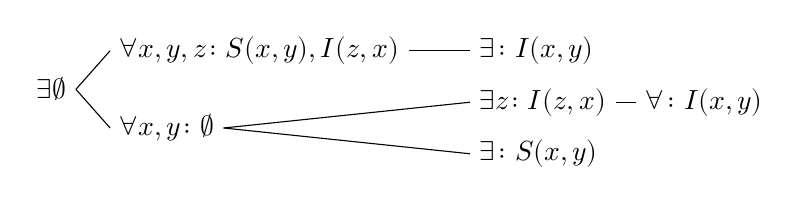
\begin{tikzpicture}
\tikzset{grow'=right}
%\tikzset{execute at begin node=\strut}
%\tikzset{level distance=70pt}
\tikzset{level 1/.style={level distance=30pt}}
\tikzset{level 2/.style={level distance=130pt}}
\tikzset{level 3+/.style={level distance=60pt}}
\tikzset{every tree node/.style={align=left,anchor=west}}
\Tree [. $\exists\varnothing$ [. $\forall x,y,z\colon S(x,y),I(z,x)$ $\exists\colon I(x,y)$ ] [. $\forall x,y\colon\varnothing$ [. $\exists z\colon I(z,x)$ $\forall\colon I(x,y)$ ] $\exists\colon S(x,y)$ ] ]
\end{tikzpicture}
\end{block}
\end{frame}

%%----------Methods----------
\begin{frame}

\frametitle{Further development of the conversion engine}
The algorithm and the software is being developed further.
\begin{block}{}
  \begin{itemize}
  \item Adaptation to TPTP syntax;
  \item Conjunctive Normal Form (CNF) support;
  \item Reconstruct the heuristic structure of CNF;
  \item Implement it in Rust programming language as it
    \begin{itemize}
    \item does not include a garbage collector in compiled code;
    \item supports a strong memory control technique;
    \item has reasonable compatibility with C and C++.
    \end{itemize}
  \end{itemize}
\end{block}
We already have a version of the algorithm for CNF having no existential variables.
\end{frame}

\begin{frame}
\frametitle{Results of prover development}
TPTP. www.tptp.org
We developed a D-language version of prover, where implemented
\begin{enumerate}
\item memory data sharing;
\item two indexing techniques;
\item basic support of simple constraints and strategies;
\item connection to outer world via Python classes;
\item tested on all FOL theorems from TPTP library.
\end{enumerate}
\end{frame}

\begin{frame}
\frametitle{TPTP test results}
\begin{block}{Total number of solved problems}
\begin{longtable}{|p{0.35\linewidth}|p{0.25\linewidth}|p{0.15\linewidth}|}
\hline
\textbf{Complexity} & \textbf{Total number} & \textbf{Solved} \\
\hline
\endhead
0,0-0,03 & 192 & 181 \\
\hline
0,04-0,20 & 435 & 373 \\
\hline
0,21-0,32 & 128 & 79 \\
\hline
0,33-0,49 & 115 & 44 \\
\hline
0,5-0,67 & 223 & 21 \\
\hline
0,68-0,92 & 72 & 6 \\
\hline
0,93-1,0 & 56 & 0\\
\hline
\end{longtable}
\end{block}
Our rating is about 0,1--0,15.
\end{frame}

\begin{frame}
  \frametitle{Testing results}
  \begin{block}{Results by domains}
    \begin{longtable}[H]{|l|p{0.2\linewidth}|p{0.15\linewidth}|}
\hline
\textbf{Domain} & \textbf{Total number} & \textbf{Solved} \\
\hline
Geometry (GEO) & 242 & 204 \\
\hline
Management (MGT) & 22 & 22 \\
\hline
Syntax (SYN) & 275 & 180 \\
\hline
Semantic web (SWB) & 25 & 22 \\
\hline
\end{longtable}
\end{block}
\begin{block}{Most complex solved (not checked)}
  \begin{longtable}{|p{0.3\linewidth}|p{0.2\linewidth}|p{0.15\linewidth}|p{0.2\linewidth}|}
\hline
\textbf{Problem} & \textbf{Complexity} & \textbf{Time,s} & \textbf{Step count} \\
\hline
%\hline
%LCL662+1.005 & 1,0 & 1,02 & 7772 \\
LCL652+1.015 & 0,92 & 32,1 & 185\,{}253 \\
\hline
LCL656+1.020 & 0,92 & 1,24 & 845 \\
\hline
\end{longtable}
\end{block}
\end{frame}

\begin{frame}

\frametitle{Research target: Logical-dynamic imitation modeling}

\begin{figure}
\includegraphics[width=0.7\linewidth]{pics/elevbetter}
\end{figure}
\vspace{-4em}
\begin{enumerate}\small
\item Intuitionistic inference in non--Horn formalization.
\item Utilization of prover engine in forward-chaining inference.
\item Constraint satisfaction.
\item Independent mostly asynchronous inference.
\end{enumerate}
\end{frame}


%%----------application------------
\begin{frame}

\frametitle{Conclusion}
The software development of method of the PCF has a number of challenges, which are under research, but the progress we made shows that the inference method is meaningful to research further.
\begin{block}{}
  \begin{itemize}
  \item Something different to Resolutional methods and Tabbling;
  \item It has direct technical origins (Theory of Control);
  \item Constructive inference of non--Horn clauses;
  \item Heuristic structure presentation.
  \end{itemize}
\end{block}
\end{frame}
  \maketitle
\end{document}


%%% Local Variables:
%%% mode: latex
%%% TeX-master: t
%%% TeX-engine: pdftex
%%% End:
